\section{The Simulation}
In contrast to the large scale threshold analysis done by \citet{OGorman2016} this work focuses on the physical simulation of the building block of the surface code error detection - the stabilizer measurements which is done by measuring the parity of a group of qubits. On the smallest scale this is given by a group of four data qubits and one probe/ancillary qubit as shown in fig.\@ \ref{FIG:paper-parity}. 

\subsection{The dipole-dipole interaction}\label{sec:dipole-dipole}

The interaction of the orbiting ancillary qubit with each data qubit is governed by the Hamiltonian

\begin{equation*}
H = \mu_B B( g_1 \sigma_1^Z + g_2 \sigma_2^Z) + \frac{J}{r^3} ( \mathbf{\sigma_1} \cdot \mathbf{\sigma_2} - 3 ( \hat{\mathbf{r}} \cdot \mathbf{\sigma_1}) ( \hat{\mathbf{r}}\cdot \mathbf{\sigma_2})).
\end{equation*}

First of all, there is the Zeeman part which accounts for the energy of each spin (data and probe) in an external magnetic field. The second interaction term is of magnetic dipole-dipole type with the interactions strength $J=\frac{\mu_0 g_e^2 \mu_B^2}{4\pi}$ and $\hat{\mathbf{r}}$ is the unit vector between the two spins. The magnetic dipole-dipole interaction is of long range compared to proposals based on the exchange interaction \cite{Kane1998a} which makes this approach very attractive as it reportedly lowers the enormous requirements on the qubit placement precision as shown by \citet{OGorman2016}. Nevertheless, the interaction scales with $1/r^3$ which makes a data to probe qubit distance on the order of several tens of nanometres necessary to achieve a strong interaction. In order to avoid crosstalk between the data qubits in the plane the lattice spacing $D$ of the data qubits should be at least one order of magnitude larger than the data and probe spacing $d$. 

Our goal is to achieve a parity measurement using this interaction. The dipole-dipole term allows us to perform a controlled phase gate between the data and probe qubit which is shown in \cite{OGorman2016} and can be seen from the dependence on both spin matrices $\mathbf{\sigma_1}$ and $\mathbf{\sigma_2}$. This means that depending on the data qubit state the probe qubit evolves in a different direction on the bloch sphere, acquiring a measurably different phase. 

In order to simulate the time evolution of both qubits under the effect of this Hamiltonian by solving the Schr\"odinger or master equation, we need to transform into the interaction picture and apply the rotating wave approximation. This allows us to get rid of the fast dynamics governed by the Zeeman term while maintaining the physical interaction which we are interested in. In our work simulations have been done using the master equation solver provided by the QuTiP library in Python \cite{Johansson2012,Johansson2013}.

In this approximation the interaction Hamiltonian is

\begin{align*}
	H_{int}&= \frac{J}{r^3} (1-3 \cdot \hat{r}_z^2) \cdot
	\begin{pmatrix}
	1 & 0 & 0 & 0 \\
	0 & -1 & 0 & 0 \\
	0 & 0 & -1 & 0 \\
	0 & 0 & 0 & 1 
	\end{pmatrix} \\
	&+ \frac{J}{r^3} (2-3 \cdot \hat{r}_x^2 -3 \cdot \hat{r}_y^2) \cdot
	\begin{pmatrix}
	0 & 0 & 0 & 0 \\
	0 & 0 & e^{-4 \Delta i} & 0 \\
	0 & e^{4 \Delta i} & 0 & 0 \\
	0 & 0 & 0 & 0 
	\end{pmatrix}
\end{align*}
where $\Delta=\mu_B B (g_1-g_2)$. Depending on the relation between $\Delta$ and $J/r^3$ the interaction will have a different character. 
To achieve a controlled phase gate on the probe qubit while keeping the data qubit unchanged we want to be in the regime where $\Delta \gg J/r^3$.
In order to estimate what orders of magnitude we require to achieve this we performed simulations for various magnitudes of $\Delta d^3/ J$ where $d$ is the minimal interaction distance as shown in fig.\@ \ref{FIG:paper-parity}.

\begin{figure}[H]
	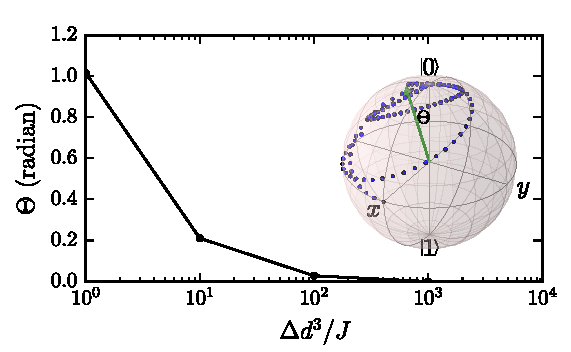
\includegraphics[width=\linewidth]{../Figures/flip-flop}
	\caption{Quantifying the flip-flopping character of the dipole-dipole interaction. For small $\Delta d^3/ J$ (see inset) we observe strong flip-flopping of the data and probe qubit which we show by plotting the maximum angle $\Theta$ which the data qubit (initialised in $\ket{0}$) takes throughout the evolution. We require $\Delta d^3/ J > 10^4$ to preserve the data qubit state.}
	\label{FIG:flip-flop}
\end{figure}

When $\Delta = J/d^3$ we observe a strong flip-flopping behaviour between the data (initialised in $\ket{0}$) and probe qubit (initialised in $\ket{+}$) as shown in the inset of fig.\@ \ref{FIG:flip-flop}. We want to avoid any change of the data qubit state. To quantify the flip-flopping we plot the angle $\theta$ the data qubit evolves for a given time for different magnitudes of $\Delta d^3/ J$ (see fig.\@ \ref{FIG:flip-flop}). Flip-flopping vanishes for $\Delta d^3/ J > 10^4$ preserving the data qubit state. This is achieved by using different species of qubits for the data and probe lattice (see Table.\@ \ref{TAB:qubits}).

\subsection{The parity measurement}
Having identified the regime where the dipole-dipole interaction performs a controlled-phase gate, we move on to the demonstration of a parity measurement.

The parity measurement should report `even' when the number of data qubits pointing up and pointing down is even. And it should report `odd' when the number of data qubits pointing up and pointing down is odd.

Realising a parity measurement using the controlled-phase gate is done by initialising the probe qubit in the $\ket{+}$ state and timing the interacting of the probe qubit with every data qubit such that the probe qubit acquires a controlled phase of $\pi/2$ for every data qubit. For even parity the probe qubit will evolve back into the $\ket{+}$ state (see fig.\@ \ref{FIG:even} for the case of all four qubits being initialised in $\ket{0}$) while odd parity evolves the probe qubit to the $\ket{-}$ state (see fig.\@ \ref{FIG:even} where one of the four qubits has been initialised in $\ket{1}$). The parity is therefore obtained by measuring the probe qubit in the $x$-basis.    


\begin{figure}[H]
	\subfloat[]{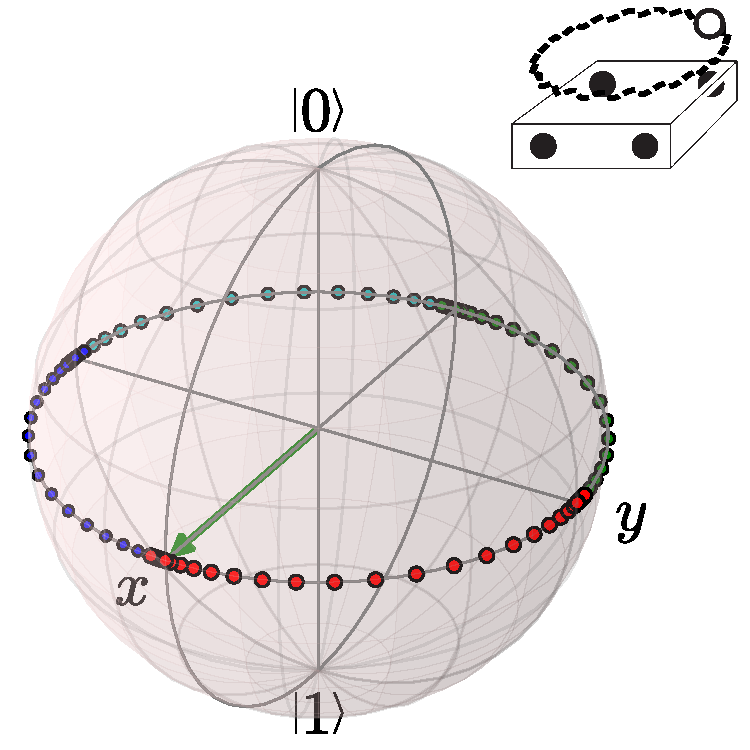
\includegraphics[width=0.49\linewidth]{../Figures/perfect_evolution_even_edit} \label{FIG:even}}
	\subfloat[]{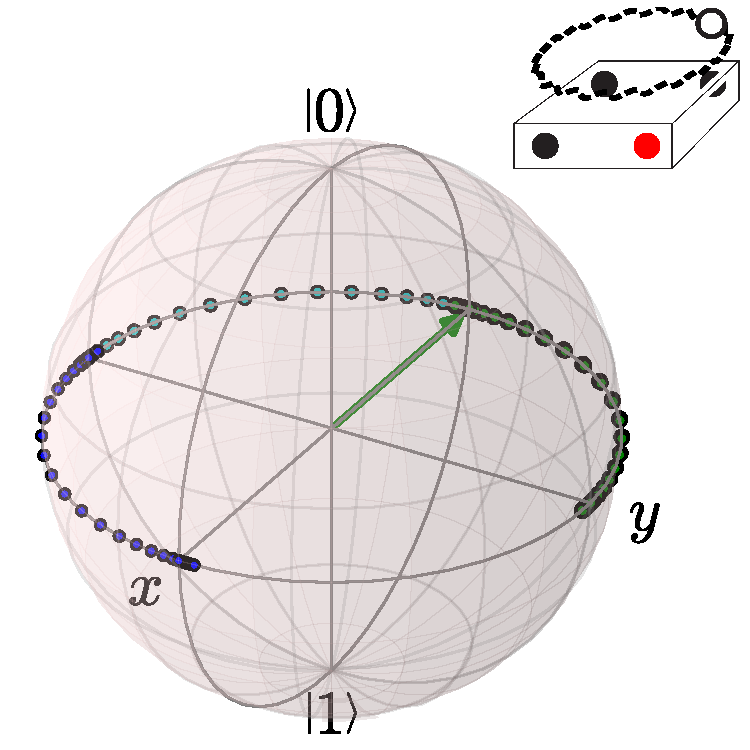
\includegraphics[width=0.49\linewidth]{../Figures/perfect_evolution_odd_edit} \label{FIG:odd}}
	\caption[oddeven]{Demonstration of the parity measurement using the controlled  $\pi/2$ phase gate and initialisation of the probe qubit in the $\ket{+}$ state. (a) All data qubits are initialised in the $\ket{0}$ state (black) representing an even parity configuration. The probe qubit undergoes a $2\pi$ evolution back to  the $\ket{+}$ state. (b) Now the last qubit is initialised in the $\ket{1}$ state (red). As a result of this the probe qubit evolves into the $\ket{-}$ state. Any other odd or even configuration will result in the same final state. The parity is extracted by measuring the probe qubit in the $x$-basis. The four different colours indicate the interaction with the four data qubits.}
	\label{FIG:evolution}
\end{figure}


The orbit which the probe qubits take to perform the parity measurement can take any possible form. Our simulations include an abrupt movement where the probe qubit jumps directly from one data qubit to the next and so on (see fig.\@ \ref{FIG:paper-abrupt}). This is very unphysical but describes the optimal orbit as it reduces the measurement time to a minimum. In addition we simulate a circular orbit with a constant speed (see fig.\@ \ref{FIG:paper-circ}). An intermediate orbit between these two cases will most likely be implemented in an experiment. 

The time each data qubit should interact with the probe qubit to realise a controlled $\pi/2$ rotation in the bloch sphere is obtained by varying the interaction time while monitoring the phase acquired by the probe qubit. This is done for every chosen orbit and an exemplary simulation is shown in fig.\@ \ref{FIG:get_tau} for the abrupt orbit. A rotation of $\pi/2$ is achieved for $\tau\approx \SI{77}{\micro s}$.


\begin{figure}[H]
	\begin{minipage}[t]{0.15\linewidth} 
	\subfloat[]{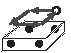
\includegraphics[width=\linewidth]{../Figures/abrupt} \label{FIG:paper-abrupt}}\\
	\subfloat[]{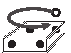
\includegraphics[width=\linewidth]{../Figures/circ} \label{FIG:paper-circ}}
	\end{minipage}
	\subfloat[]{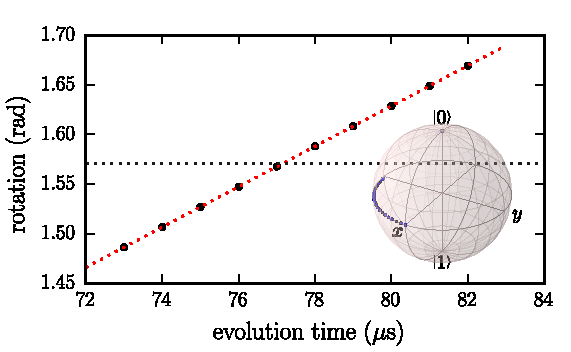
\includegraphics[width=0.85\linewidth]{../Figures/abrupt_find_tau_full.pdf} \label{FIG:get_tau}}
	\caption{(a) Schematic of the abrupt orbit. Direct copy from \cite{OGorman2016}. (b) Schematic of the circular orbit. Direct copy from \cite{OGorman2016}. (c) We obtain the optimal interaction duration to implement a $\pi/2$ rotation by varying the evolution time while monitoring the phase acquired by a probe qubit initialised in the $\ket{+}$ state. Here we show the example of the abrupt orbit with $d=40\, $nm and we find $\tau\approx \SI{77}{\micro s}$.}
	\label{FIG:abrupt_tau}
\end{figure}

In order to estimate the time a parity measurement would take in an experiment, we determine the parity measurement time for the abrupt and circular orbit for several data and probe qubit separations $d$ and data qubit lattice spacings $D$.

\begin{figure}[H]
	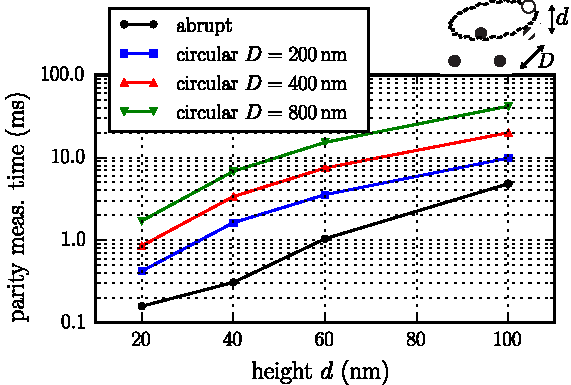
\includegraphics[width=\linewidth]{../Figures/tau_d_D}
	\caption{Simulation of the overall parity measurement time for the abrupt and circular orbit with various qubit lattice constants $D$ and probe and data qubit layer separation $d$.}
	\label{FIG:tau}
\end{figure}

The shortest parity measurement time $\tau=\SI{158}{\micro s}$ is achieved with the abrupt motion ($d=20\, $nm).
The parameter $d$ has the strongest influence on the parity measurement time due to the $1/r^3$ dependence of the interaction.
For a reasonable experimental implementation, we expect the parity measurement to be of the order of several milliseconds.


\subsection{Spin species}

Having demonstrated how the parity measurement is realised and how long each measurement could take we now look into different available spin systems. 

As shown in the previous sections we require $\Delta d^3/ J > 10^4$. This is achieved by choosing two different spin species for the data and probe qubits. Any sensible combination of species given in Table.\@ \ref*{TAB:qubits} fulfils this criterion.

For the data qubits we desire qubits with long coherence to maintain the quantum information throughout a large number of parity measurements. Furthermore, we only require global control for the data qubits during operation as logical operations on the encoded qubits can be performed using the stabilizer measurements.
In case of the probe qubits we require coherence times which are longer than the time it takes to perform a parity measurement. In addition to that readout is very important and individual control is required.


\begin{table}[H]
	\begin{tabular}{lrrrr}
		\hline
		spin qubit & $T_1$ & $T_2^{*}$ & $T_2$ & $T_{2,\textrm{decoupl}}$ \\ \hline \\
		P (nat. Si, mK, SET) \cite{Pla2012}& $0.7\, $s & $^{10}55\, $ns  & $^5206\, \si{\micro s}$ & $410\, \si{\micro s}$  \\
		P ($^{28}$Si, mK, SET) \cite{Muhonen2014}&  & $^7160\, \si{\micro s}$  & $^41\, $ms & $560\, $ms \\
		P$^{\text{nuc}}$ ($^{28}$Si, mK, SET) \cite{Muhonen2014}& & $500\, \si{\micro s}$ & $1.75\, $s & $35.6\, $s \\
		P ($^{28}$Si, $6.9\, $K, bulk) \cite{Morley2010}& &  & $14\, $ms &  \\
		P ($^{28}$Si, $1.8\, $K, bulk) \cite{Tyryshkin2011}& &  & $0.6\, $s &  \\
		Bi ($^{28}$Si, $4.3\, $K bulk CT) \cite{Wolfowicz2013} & $9\, $s &  & $^12.7\, $s &\\
		NV ($^{12}$C, RT) \cite{Balasubramanian2009,Bar-Gill2013} & & & $^21.8\, $ms & $3.3\, $ms \\
		NV ($^{12}$C, $77\, $K) \cite{Bar-Gill2013} & & &  & $0.6\, $s \\
		SiC ($20\, $K) \cite{Christle2014} & & $^81.1\, \si{\micro s}$ & $^31.2\, $ms &  \\
		SiC (RT) \cite{Koehl2011} & $185\, \si{\micro s}$ & $^9214\, $ns & $^640\, \si{\micro s}$ &   \\
		\hline
	\end{tabular} 
	\caption{Summary of coherence times of various spin qubit systems. The spin species as well as the measurement temperature is given. RT stands for room temperature while CT refers to clock transitions. For donors in Silicon we distinguish between near surface dopants read out using a single-electron-transistor (SET) and bulk dopants. The numbers in superscript refer to fig.\@ \ref{fig:phaseplot}.}
	\label{TAB:qubits}
\end{table}

This illustrates that coherence is an important parameter for choosing a spin system. Dephasing is a reversible loss of coherence due to inhomogeneous broadening which is characterised by the dephasing time $T_2^*$ which is usually much shorter than a millisecond (see Table.\@ \ref{TAB:qubits}). Luckily we should be able to combine the parity measurement with spin echo or even dynamical decoupling techniques enhancing coherence to the more generous time $T_2$ which represents irreversible loss of coherence.

Donors in silicon are excellent candidates for both data and probe qubits as they offer extremely long coherence times when implanted in purified $^{28}$Si (see Table.\@ \ref{TAB:qubits}). Moreover, electrical read out of high-fidelity using a single-eletron-transistor (SET) \cite{Pla2012,Pla2013,Muhonen2014} as well as optical \cite{Lo2015} read out has been demonstrated for $^{31}$P donors and is feasible for $^{209}$Bi. Control of individual spins can be achieved by tuning them in and out of resonance using the stark effect \cite{Pica2014}. The control electronics has a small footprint making a large scale implementation feasible. Being able to transfer the electron spin state to the nuclear spin offers even longer coherence times. Additionally, $^{209}$Bi has several clock transitions (CT) which are insensitive to magnetic fields leading to very long electron spin coherence times ($T_2=2.7\, $s). However, operation in this regime will make the $^{209}$Bi qubit also insensitive to the magnetic dipole-dipole interaction. Tuning in an out of the CT will be necessary to implement the parity measurement. Proof-of-concept implementations could benefit from that fact that donors in silicon even offer moderate coherence times at elevated temperatures. However, the coherence times demonstrated in bulk still remain to be reproduced for near-surface donors as required for this scheme.
Finally, MEMS devices with a sensitivity of \SI{25}{\hertz\per nm} and $0.3\, $nm accuracy \cite{Chu2003} as well as an accuracy of $5\, $nm with a bandwidth of $30\, $Hz have been demonstrated. This gives good prospects for realisation of highly accurate and fast MEMS devices as needed for this scheme in the near future. 

Besides donors in Si we imagine nitrogen vacancies (NV) to be a promising candidate for proof-of-concept demonstrations. NV centres are highly developed qubits \cite{Bar-Gill2013} which offer good coherence times even at room temperature (RT) \cite{Balasubramanian2009}. Individual addressing can be achieved using the stark effect. Optical read out and the possibility of integrating NV centres into an atomic force microscope (AFM) tip makes NV centres good candidates for a probe qubit \cite{Grinolds2013}. The optical read out of NV centres has one drawback as the readout frequency excites carriers in silicon. As a result of this read out has to be performed carefully in safe distance to the data qubits. Additionally diamond MEMS devices still need to be demonstrated.

Recently, defects in SiC have attracted lots of attention \cite{Morello2015} as coherent manipulation of individual spins with predicted room temeprature coherence times on the order of milliseconds has been demonstrated \cite{Widmann2014}. At cryogenic temperatures ($20\, $K) this has already been achieved \cite{Christle2014}. Current experiments still suffered from a low collection efficiency. Having near infra-red transitions, SiC shows excellent prospects for integration with optical fibres. Moreover, AFM tip integration is feasible. However, SiC is still at a very early research stage.  


 
